\documentclass[12pt, twoside]{report}
% https://www.overleaf.com/learn/latex/How_to_Write_a_Thesis_in_LaTeX_(Part_1)%3A_Basic_Structure
\usepackage[utf8]{inputenc}
\usepackage{graphicx}
\graphicspath{{images/}}
\usepackage{amsmath, amssymb}
\usepackage[a4paper, width=150mm, top=25mm, bottom=25mm, bindingoffset=6mm]{geometry}
\usepackage{fancyhdr}
\pagestyle{fancy}
\usepackage[backend=bibtex, style=alphabetic]{biblatex}
\addbibresource{references.bib}
\usepackage[dvipsnames]{xcolor}
\usepackage{listings}
\definecolor{codegreen}{rgb}{0,0.6,0}
\definecolor{codegray}{rgb}{0.5,0.5,0.5}
\definecolor{codepurple}{rgb}{0.58,0,0.82}
\definecolor{backcolour}{rgb}{0.95,0.95,0.92}
\lstdefinestyle{mystyle}{
    backgroundcolor=\color{backcolour},   
    commentstyle=\color{codegreen},
    keywordstyle=\color{magenta},
    numberstyle=\tiny\color{codegray},
    stringstyle=\color{codepurple},
    basicstyle=\ttfamily\footnotesize,
    breakatwhitespace=false,         
    breaklines=true,                 
    captionpos=b,                    
    keepspaces=true,                 
    numbers=left,                    
    numbersep=5pt,                  
    showspaces=false,                
    showstringspaces=false,
    showtabs=false,                  
    tabsize=4
}
\lstset{style=mystyle}



\title{
    {GPU code optimisations and the tree reduction algorithm} \\
    {\large University of Regensburg} \\
    {
\includegraphics[width = 0.5\textwidth]{ur_logo.jpg}}
}
\author{Tobias Sizmann}
\date{30th April, 2023}

\begin{document}

\maketitle

\tableofcontents

\chapter{Introduction}
\section{From single-core CPUs over multi-core CPUs to GPUs}

\begin{figure} \label{fig_tree_reduction}
    \centering
    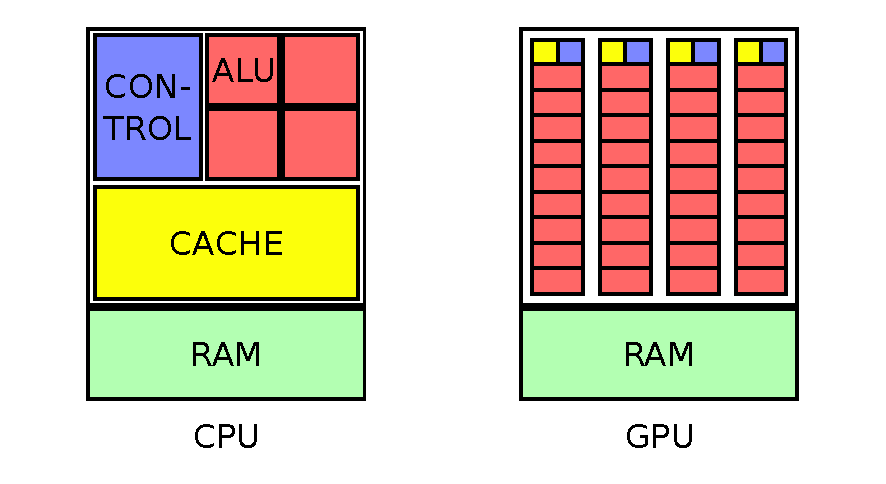
\includegraphics[]{cpu_vs_gpu.pdf}
    \caption{
        Comparison of the basic architectural differences of a GPU and a CPU.
        In green the random access memory (RAM), in yellow the cache, in blue the flow control unit and in red the arithmetic-logic unit (ALU).
        Both designs feature a RAM that all threads have access to.
        The GPU is split into many small "CPUs" (vertical groups) with their own flow control and cache.
        These are called streaming multiprocessors (SMPs or SMs).
        Generally the cache hierachry is more complicated as depicted in the figure.
        However, the defining property here is that there exists a non-global cache level that is assigned to a group of ALUs, namely the SMs. 
        Note that the notion of an ALU has slightly different meaning for a CPU and a GPU.
        For a CPU one ALU usually corresponds to one thread.
        For a GPU one ALU usually corresponds to a group of threads (for modern GPUs: 32), called a warp.
    }
\end{figure}

With the invention of the MOS transistor in 1959 and more specifically the silicon-gate MOS transistor in 1968 the development of single-chip microprocessors started.
The first processors were single-threaded and their bottleneck was (besides other things) their clock rate.
However, clock rates increased exponentially over time and subsequentially did the computing power.
In the 2000s this development was eventually brought to a halt at around 3.4 GHz due to thermodynamical limits of silicon. 
While pushing past that limit is possible, the extra costs for cooling usually outweight the increase in computing power.
This is the beginning of the multiprocessing era. 
The idea is simple: When one thread cannot run faster, just increase the number of threads.
In 2006 the first desktop PCs with two cores were sold and ever since the number of threads is steadily increasing.
There was one problem in particular, however, that CPUs (Central Processing Unit) were not efficient in solving, namely, rendering graphics.
This task required a lot of independent and small calculations that needed to be done in real time - a prime example for a massively parallelisable computation.
Since rendering graphics required such a different type of computing, the first GPUs (Graphics Processing Unit) were developed.
These GPUs featured less single thread computation power but have a higher number of threads.
State of the art GPUs have thousands of threads.
This being said, the number of threads cannot be easily compared between a CPU and a GPU or even between different GPUs as they follow different design paradigms.
How the GPU threads work exactly will be explored in this work.
Generally, one can say that GPUs perform well in massively parallelisable computations where the single computations are not complex while CPUs excel at complicated single threaded problems (for example running the event loop of a desktop application).
This shift to a higher number of threads rather than thread quality has been greatly motivated by scientific calculations, machine learning and graphics.

In this work, the basics of GPU programming in CUDA will be introduced and a very important algorithm presented, namely the tree reduction.
Using this algorithm as an example, a deeper look into the architecture of GPUs and the CUDA programming language will bring forth various optimisations.
Finally, the highly optimized implementation of the tree reduction will be tested on a consumer grade setup and a high-performance computer and the results will be discussed.

\section{What is CUDA}
Writing code for a GPU is not as straight forward as for a CPU since it is more dependent on its hardware.
Different GPU developers use different application programming interfaces (APIs).
The biggest GPU designer Nvidia developed a framework called CUDA, which will be used in this work.
It is simple to learn, offers efficient implementations and a plethora of literature and support.
The downside is that it only supports Nvidia GPUs and is not open-source.
An alternative would be OpenCL, which is open-source but harder to learn, or HIP, which is the CUDA equivalent by AMD and very similar to it.

CUDA works as an extention to the C programming language and comes with its own compiler.
Sections of code are distributed to either the CPU (called host) or the GPU (called device).
When only writing code for the host normal C is used.
Writing device code is more sophisticated.
Here, the programmer first needs to write a so called kernel, which can be thought of the interior of a for-loop.
Then the host must transfer required data to the memory of the GPU and call the kernel.
When calling the kernel, the boundaries of the for-loop are set.
The loop is then executed in parallel on the GPU.
This API only allows parallelisation of for-loops.
While this might seem like a very strict limitation, it closely relates to how a Nvidia GPU works.

The GPU can be thought of being organised in streaming multiprocessors (SMPs or SMs), warps and threads.
Warps will be explained in more detail later.
A SM groups together a set of (hardware) threads and allows synchronisation between them.
Threads of different SMs cannot be synchronised.
Also, threads within a SM share a cache, which cannot be accessed by threads of another SM.
The domain of the for-loop is organised in blocks and (CUDA) threads, where the threads are grouped in blocks.
The blocks are executed by the SMs, which means that only threads within a block can be synchronised and have access to the same cache.
Note the differentiation of hardware and CUDA threads.
This is an unfortunate ambiguity in the terminology of CUDA.
While each CUDA thread is mapped to one hardware thread, a hardware thread can be mapped to (i.e. execute) several, none or one CUDA threads.
This will become clearer in the next chapter.


\chapter{Tree Reduction on GPUs}
\section{The importance of reductions}
A reduction in terms of parallel programming is an operation where a large dataset of entries (e.g. numbers) is reduced to one entry.
The simplest example is the sum of a set of numbers and will be used for the rest of this work.
More generally a reduction is defined by an operation \( \circ: X \times X \rightarrow X \) on two entries with the following properties:
\begin{align}
    a \circ b &= b \circ a \ \ \mathrm{(commutativity)}, \\
    a \circ (b \circ c) &= (a \circ b) \circ c \ \ \mathrm{(associativity)}.
\end{align}
This guarantees that the result is (mathematically) independent of the order in which the elements are reduced.
Note, that these properties do not ensure numerical stability.

The reduction operation, first and foremost the sum, plays a crucial role in all of numerics.
Even simple linear algebra operations like the scalar product or the matrix multiplication already include a reduction:
The entries of two vectors are multiplied element wise and then summed up.
In machine learning, reductions are present as a key step in feed-forward networks:
Again all the values of the node one layer below are multiplied by weights element wise and then summed up to calculate the value of a single node above.
Reductions are a very basic and fundamental operation and, therefore, an efficient implementation is required. 

\section{The tree reduction algorithm}
\begin{figure}
    \centering
    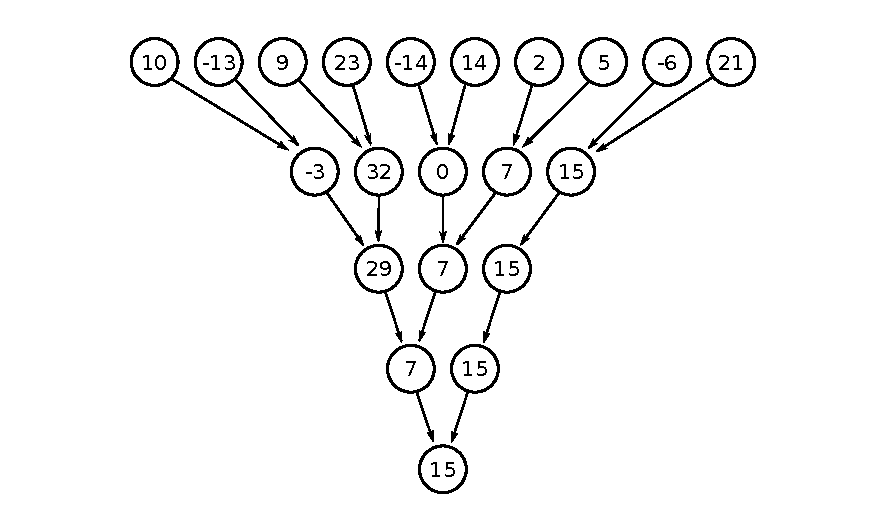
\includegraphics{tree_reduction.pdf}
    \caption{
        Example of a tree reduction of ten elements.
        Note how there is a leftover after the first reduction.
        These are usually handled by zeropadding (i.e. adding zeros) after each step to make the number of elements divisible by 2.
    }
\end{figure}
The most efficient (shortest execution time) algorithm is heavily dependent on the underlying hardware.
For example, a node network with a lot of parallelization overhead and a complicated communication topology might use a ring algorithm ("add value and pass to next thread/node").
In this work the focus is on single GPU reductions.
Here, the tree reduction approach is the most successful.
All available threads are called in parallel to each reduce two entries, effectively halving the size of the dataset in one step.
This is repeated until only one entry remains.

\section{Naive implementation with CUDA}
For a better understanding of the CUDA framework and tree reduction algorithm an unoptimized code is presented which implements the algorithm for the case of addition of signed 32-bit integers. 
Note, that even though this is unoptimized GPU code, it runs magnitudes faster than on a CPU (exact speedup depending on the problem size and the available hardware).

When approaching a problem using CUDA the big challenge is to map the for-loop that one wants to parallelize to blocks and CUDA-threads. 
Often, the best starting point is to write serial CPU code to get a feeling for the problem and to have a working solution to test the optimized solutions against later.
In this case, we will first implement a serial tree reduction in C and port this code to CUDA in a second step.

\subsection{Serial tree reduction on a CPU}
\begin{figure}
    \centering
    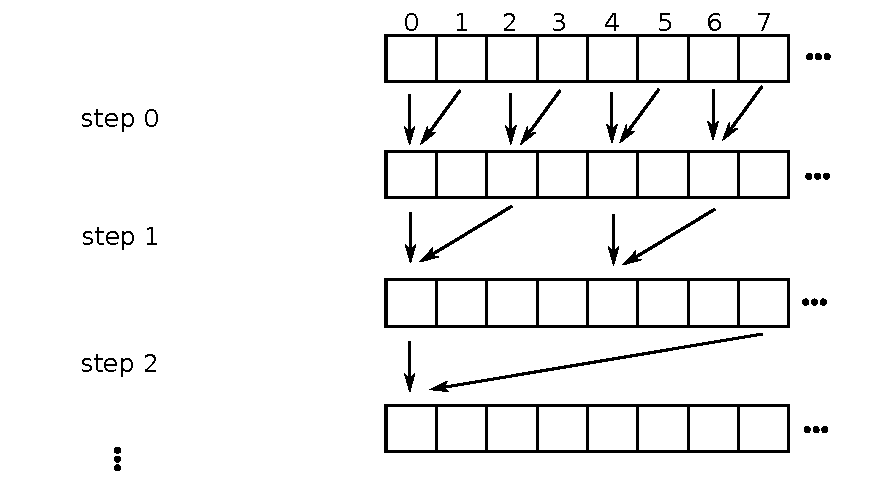
\includegraphics{naive_reduction.pdf}
    \caption{
        Sketch of the implementation of the tree reduction algorithm presented in this section.
        The cells denote entries in the data array.
        Two arrows pointing into a cell denote addition of the source cells values and writing of the result into the target cell.
        The final result is found in the first cell of the array.
    } \label{fig_naive_reduction}
\end{figure}
Our starting point is an integer array \texttt{h\_in}.
The \texttt{h\_} denotes data stored on the host (CPU RAM), which is a useful convention, since CUDA does not distinguish between pointers to host and device memory.
For simplicity, we assume that the size of the array is a power of two.
If this is not the case, one could simply zero-pad the data and would still be able to use the code.

Let's write a function \texttt{reduce} that executes the tree reduction.
This function takes an input array \texttt{h\_in}, performs the reduction and writes the result to an output \texttt{h\_out}. 
We need two for-loops:
One to iterate over the step of the reduction (vertically in Fig. \ref{fig_naive_reduction}) and one to iterate over the (remaining) data set (horizontally). 
A temporary array is used to perform the reduction on, so the input array stays untouched.

\lstinputlisting[language=C]{code/host_reduce.c}

Note that the \texttt{memcpy} function call could be avoided, but ports nicely to GPU code later on, which is the reason why it was used.
The inner loop of this implementation could be parallelized easily, since each step of the inner loop is independent.
This means, however, that with each step of the outer loop all threads are created and destroyed, which leads to a large parallelization overhead.
While this parallelization overhead can be avoided on CPUs using persistent threads, there is another solution that ports nicely to GPU code later on.
The outer loop cannot be parallelized, since each step is dependent on the result of the step before.
To fix this, one can swap the two loops.
While this requires slightly more code, it greatly simplifies all examples in the following.
The rewritten function looks like this:

\lstinputlisting[language=C]{code/host_reduce_swapped_loops.c}

Note that an additional if-statement is required.
This is a much better basis for parallelization, since now the outer loop can be parallelized.
However, one needs to be very careful as this is now prone to a race condition.
The parallelization with CUDA is done in the next section.

It should be noted, that there are much faster ways to implement a reduction algorithm as a single-thread CPU application.
This code has been written with the intent of parallelization on a GPU and serves solely this purpose.

\subsection{Tree reduction in CUDA for small arrays}
Once the algorithm has been successfully implemented serially, the parallelization of the target for-loop is always the same.
One needs to map the domain of the for-loop (here integers from \texttt{0} to \texttt{len-1}) to threads.
The maximum number of threads \( n_{\mathrm{Threads}} \) a block can contain depends on the hardware, but is always a power of two.
Nvidia GPUs with compute capability of 2.0 or higher will allow for \( n_{\mathrm{Threads}} = 1024 \) (e.g. RTX 30xx series and A100, see \cite{programming_guide}), but it is not necessarily optimal to use all threads.
This will be explored later.
For now we will restrict the maximum size of our input array to 1024, such that only one block is required.
With this, one can write down the kernel (terminology for a function running on the GPU).

\lstinputlisting[language=C]{code/device_small_kernel0.cu}

There are several things to uncover here. First, the \texttt{\_\_global\_\_ void} declares the function as a kernel, which runs on the device but can be invoked from the host. 
Secondly there is a new constant \texttt{threadIdx.x} available within the kernel.
This is an identifier of the thread that is executing the kernel.
It is unique for all threads within a block and ranges from \texttt{0} to \texttt{numThreadsPerBlock - 1}.
This replaces the index which the for-loop iterates over.
The temporary array can be replaced by the ultra-fast cache shared by all threads of one block, which is allocated during kernel invocation and declared within the kernel by the line

\lstset{firstnumber = 5}
\lstinputlisting[language=C]{code/shared_memory_line.cu}
\lstset{firstnumber = 1}

As mentioned earlier, there is a race condition between threads, which can be solved by the \texttt{\_\_syncthreads()} method.
This method acts as a wait-for-all barrier within a block (synchronization between blocks is not possible!).
Finally, the result needs to be exported.
For this, only one thread is required, hence the if-statement.
Note that the input and output pointer names start with a \texttt{d\_}, which is not required but is a convention to mark, that these pointers live in the address space of the device.

The kernel can be invoked from the host with the following code:

\lstinputlisting[language=C]{code/kernel_invokation.cu}

First the data is copied to the device memory.
Then the kernel is invoked by the triple angled brackets syntax.
Within the brackets, the number of blocks \( n_\mathrm{Blocks} \) (so far exactly one), the number of threads per block \( n_{\mathrm{Threads}} \) and the amount of cache space are specified.
The kernel arguments are specified in parentheses.
Finally, the result is copied back to the host and the device memory is free'd.
Note that in practice one would write more code to error-check every step, assure that the correct upstream is used and optimize the copy procedure.
Nonetheless, this is a minimal working example.

The big problem with this implementation is, that it is limited to an array size of 1024, since we only use one block.
This is solved in the next section.


\subsection{Tree reduction in CUDA for arbitrary array sizes}
\begin{figure}
    \centering
    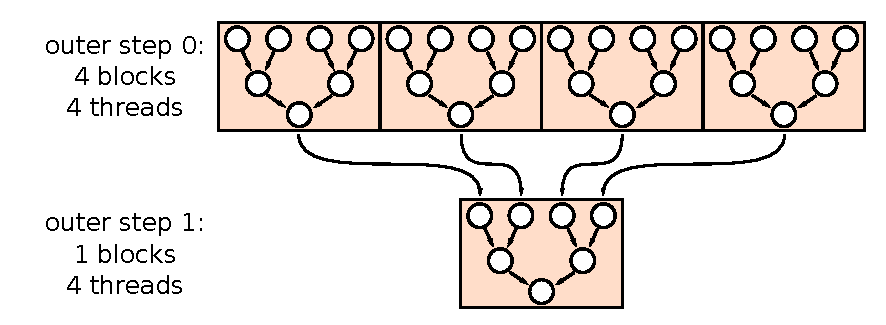
\includegraphics{block_reduction.pdf}
    \caption{
        Depicted is the schematic tree reduction in block structure for an array of length 16 and 4 threads per block.
        The first step requires 4 blocks and the second 1 block.
        The blocks run on the SMs of the GPU.
        The first step allows for four SMs and a total of 16 physical threads to be used in parallel.
        Between the two steps the output array is used as new input array.
        The second step can only make use of a single SM.
    }
\end{figure}
The limitation to an array size \( n_{\mathrm{Data}}\) of maximum block size can be solved in the following way:
Split the array into equal chunks and run the kernel on each of these chunks individually.
This procedure returns an array with size \( n_{\mathrm{Data}}/ n_{\mathrm{Threads}} \) (assuming that \( n_{\mathrm{Data}} \) is a power of 2, otherwise round up is required).
The procedure is then again used recursively, until the array is reduced to a singular value.
We refer to such a reduction step as "outer step", which reduces \( n_{\mathrm{Threads}} \) elements, compared to an "inner step" reducing 2 elements.

While this could be implemented already with the existing kernel, there is a hardware structure available to do kernel invocations with a certain amount of threads in parallel, namely the streaming multiprocessors (SMs).
The SMs are a second layer of parallelization.
One block of threads is always mapped to one SM, so several blocks can be executed in parallel on several SMs.
Unlike the number of threads per block, the number of blocks is unlimited and blocks are queued until a SM is free to work on it.
In our case this has the following implication.
Let's assume that the initial array size is \( n_{\mathrm{Data}} = n \times 1024 \).
Then one could use \( n \) blocks of 1024 threads to do the first step of the outer reduction and use the full computational power of the GPU this way.

This leaves us with a new problem, however.
Namely, how does one calculate the position of the array one specific thread is supposed to work on?
To this end, CUDA offers two more constants in the kernel:
\texttt{blockDim.x} and \texttt{blockIdx.x}.
The first one is simply the number of threads in a block and the second one is a unique identifier of the current block, ranging from 0 to \( n_{\mathrm{Blocks}} - 1\).
The array position can then be calculated with \texttt{threadIdx.x + blockIdx.x * blockDim.x}.
The required amount of blocks for the kernel invocation can be calculated with rounding up division.
This can be neatly done with \( n_{\mathrm{Blocks}} = (n_{\mathrm{Data}} + n_{\mathrm{Threads}} - 1) / n_{\mathrm{Threads}} \), where the "\( / \)" denotes integer division.

To enable the use of blocks with our kernel three small modifications need to be done.
First, the access of our input array needs to be rewritten with the new formula for the position.
Secondly, the output is not a single value but an array.
Thirdly, the range of the loop and the input array length can be deduced directly from the block size and number of threads per block and, therefore, the length of the input array does not need to be passed to the kernel.
The result from the \(i\)-th block should be written into the \(i\)-th position.
Also for simplicity the loop over the \texttt{step}-variable has been replaced by a loop over \texttt{stride} directly, saving an extra variable and the \texttt{log2} function call.
The finished code looks like this:

\lstinputlisting[language=C]{code/device_full_kernel0.cu}

The invocation changes slightly.
First, we need to specify the number of required blocks as argument in the triple angled brackets.
Secondly, the kernel has only two arguments now.
Also the size of the output array changes.

\lstinputlisting[language=C]{code/kernel_invokation_full.cu}

Note that this code only executes a single outer step of the reduction.
One would need to take the output array and feed it through this code until a single value is left.
This was left out since it is mostly host code and not of particular interest for the rest of the work.
It should be noted, however, that all code timings in the following were done for the full reduction.

\section{Conclusion}
This concludes the introduction to CUDA and tree reduction algorithms.
From now on this work focuses on modifying the kernel to optimize it as much as possible.
It should be noted, that a lot of optimization has been done already.
For example, using the explicitly declared shared memory instead of DRAM or the implementation of the block structure already offer a great speedup compared to other algorithms one could come up with.
Now, the main goal is to dive deeper into the hardware structure and achieve speedups by fixing problems like warp divergence and memory bank conflicts, which will be explained in full detail.
Some algorithmic improvements will also be done and in the end all the optimizations will be benchmarked on several hardware systems.


\chapter{Optimisations}
In this chapter various optimizations of the reduction kernel will be presented and discussed analogously to the talk by the author of \cite{Harris}.
A reduction usually (at least in the case of addition) needs very few arithmetic operations and is, therefore, bottlenecked by memory access speed.
This means that a good measure for performance is the achieved memory bandwidth rather than floating point operations per second.
Especially, if one achieves bandwidths close to the maximum of the GPU, one can consider the kernel to be optimal.
The bandwidth can be calculated using the formula
\begin{equation}
    \mathrm{bandwidth} = \frac{\mathrm{input\ array\ size\ in\ bytes}}{\mathrm{execution\ time}}.
\end{equation}
The execution is defined as only the reduction and not the copying of the data to the GPU, which is reasonable, since for most use-cases the data would already be present in the GPU memory.

All achieved bandwidths shown in this chapter will be done on a Nvidia GeForce RTX 3070 (max. bandwidth: 448 GB/s, CUDA version: 11.5) with an input array of \( 2^{28} (1.3\cdot 10^8)\) 32-bit integers. 
This is a relatively new GPU (released Q4 2020).
The GPU and the software that comes with it already have optimizations implemented that might mess with the results.
To this end, data from a Nvidia G80 (max. bandwidth: 86.4 GB/s, CUDA version: 1.1) is provided as well published by \cite{Harris}.
All measurements are done 1000 times to estimate the statistical error on the results.
The results are presented merely to give a first impression on the effectiveness of the various changes on the kernel.
In the last chapter, the performance will be investigated more closely and on several different GPUs.

\begin{center}
    \begin{tabular}{|c|c|c|}
        \hline
        GPU & G80 & RTX 3070 \\
        \hline
        Release & 2006 Q4 & 2020 Q3 \\ 
        \hline
        Max. Bandwidth & 86.4 GB/s & 448 GB/s \\
        \hline
        Compute capability & 1.0 & 8.6 \\
        \hline
        Used CUDA compiler & 1.1 & 11.5 \\
        \hline
    \end{tabular}
\end{center}

\section{Starting point: The naive kernel}
The starting point is the kernel presented in the last chapter.
In order to setup a timing routine, a wrapper was written, which executes the full reduction, i.e., it calls the kernel repeatedly with the required amount of blocks for each outer step until the reduction is fully done. 
Since the wrapper runs on the host, some of the execution time is spent on the CPU, but for large enough arrays this part becomes negligible small.
Another addition to execution time is the call to the routine \texttt{cudaMemset()} which sets the memory of the device to a specified value.
This is required for the aforementioned zero-padding.
Again, the additional execution time is negligible.
For the naive kernel a bandwidth of 127.1 (\(\pm 1.0\% \)) GB/s was measured on the RTX 3070.

\section{Divergent warps}
The first problem that needs to be dealt with is divergent warps.
The threads of a streaming multiprocessor (SM) are clustered into so-called warps or SIMD (single instruction multiple data) lanes or vectors.
Usually, one warp contains 32 threads and they are grouped with increasing \texttt{threadIdx.x}, i.e., threads 0 to 31 are one warp, 32 to 63 are one warp, etc.
These threads are always synchronized in the sense that they execute the same instruction but act on different regions of memory (hence the name SIMD).
If one thread in a warp was to execute a different instruction than the rest, which in CUDA happens through if-statements, all other threads are masked off (i.e. they still run but have no affect on memory).
This is a highly inefficient procedure! 
Consider the following worst case example:
\lstinputlisting[language=C]{code/divergent_warps_worst.cu}
Here, the first 4 threads all execute different paths, which is called divergent branching.
In order to run this code the flow control unit of the SM must first mask off all threads of the warp except the first and run those instructions, then mask off all threads except the second and run those instructions and so on.
This basically leads to the threads being executed serially rather than in parallel.
There are two ways to fix this code.
The first one is to use different blocks, i.e., use \texttt{blockIdx.x} in the if statements instead.
This has two other disadvantages though.
First, a whole SM is used to run the execution path of a single thread.
Secondly, the threads cannot be synchronized afterwards.
If one needs to add a barrier, basically a new and separate kernel invocation is required.
The better solution is to use different warps:
\lstinputlisting[language=C]{code/divergent_warps_fixed.cu}
Each of the four paths are now running on different warps and therefore in parallel.
This being said, there is still a lot of computer power wasted, since of each warp only one thread is used.
Depending on the situation, however, this might be the most optimal solution.
Usually, for highly complex branching code (e.g. an event loop of a desktop application), the CPU is preferred.
Simple branching like in this example cannot be avoided most of the time and proper warp mapping is crucial for optimal performance. 

In the case of the reduction kernel divergent warps are present which can be nicely seen in the code:
\lstinputlisting[language=C]{code/kernel0_ifstatement.cu}
During the very first inner step, the if-statement branches within a warp.
Thread 0 does some addition and thread 1 idles, thread 2 adds and thread 3 idles etc ...
This means that there are two execution branches within one warp.
If one would map all idle threads to one warp and working threads to another, then idling and adding would be executed in parallel.
This can be simply done by rewriting the for-loop:
\lstinputlisting[language=C]{code/kernel1_ifstatement.cu}
Also, the costly \texttt{\%}-operator vanishes this way.

On the RTX 3070 the new bandwidth is 176.0 (\( \pm 0.9\% \)) GB/s, which is an increase of roughly 38\%.
In theory one would expect an increase close to 100\%, and as a matter of fact, on older GPUs (Nvidia G80) with an older CUDA compiler, one actually achieves this.
The reason most likely is, that modern flow control units and compilers are able to do this optimization to some degree by themselves, which means that the naive kernel already had some sort of divergent warp prevention.
Still a 38\% increase is non-negligible.

\section{Memory bank conflicts}

\begin{figure}
    \centering
    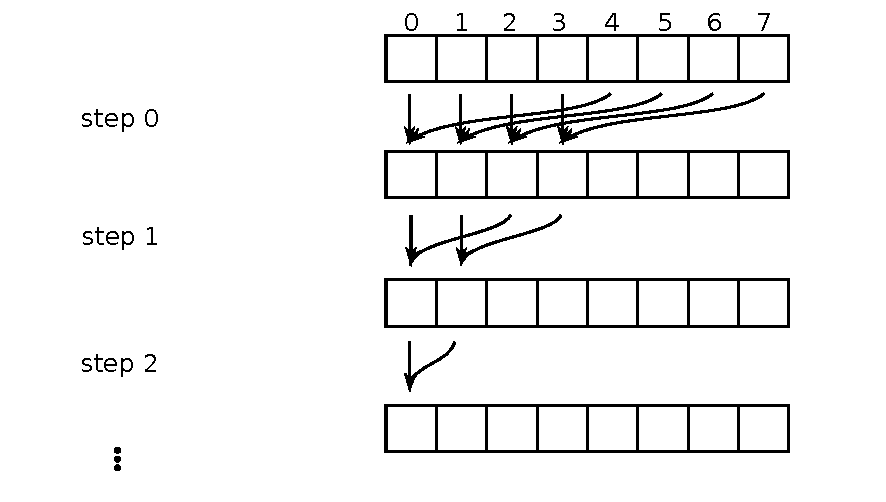
\includegraphics{coalesced_reduction.pdf}
    \caption{
        Depicted is the same algorithm as in Fig. \ref{fig_naive_reduction} for 8 elements.
        However, this time the results of the addition of two cells is written into memory, such that the data stays contiguous.
        Note that one needs to be careful not to introduce an additional race condition when accessing the elements.
    } \label{fig_coalesced_reduction}
\end{figure}

A similar problem to the divergent warps appears when accessing the ultra-fast shared cache.
This memory is divided into 32 so called memory banks where each bank has a bandwidth of 32 bits per clock cycle.
The mapping of the address space to the banks is done periodically, i.e., 
\begin{equation}
\mathrm{bank\ number} = \mathrm{address} \mod 32
\end{equation}
Two threads cannot access the same bank in the same clock cycle.
If this case appears, the warp(s) of the two threads is(are) frozen for one cycle and the memory loads/stores are done sequentially.
One exception is, when the two threads load from the same address.
In this case a broadcast operation is done, which requires no freezing.

Usually, memory bank conflicts are not completely avoidable, but should be reduced to a minimum.
This can be achieved by memory coalescing, i.e., keeping the data that is being worked on contiguous in memory.
In our case, the memory is not coalesced, which can be seen in Fig. \ref{fig_naive_reduction}.
After the first step there are "holes" in the data which is being accessed in the next step.
This effectively halves the bandwidth of the shared memory in the second step.
After the second step, it only gets worse.
The bandwidth for the third step is effectively quartered.
Since after each step the amount of data is also halved, this leads to an overall avoidable slow-down of roughly 50\%.

The solution to this problem is simple.
One needs to write the results of each addition back into memory in such a way, that the data stays coalesced.
This is depicted in Fig. \ref{fig_coalesced_reduction}.
In terms of code this requires only a slight modification to the for-loop of the kernel:
\lstinputlisting[language=C]{code/kernel2_forloop.cu}
The order of the for-loop was reversed and the thread index can be used again for accessing the array.

With this a bandwidth of 185.1 (\( \pm 1.1\% \)) GB/s was achieved on the RTX 3070, which is an increase of roughly 5\%.
Again, on the older setup with the G80 the expected speedup of 100\% was achieved.
The difference most likely stems from the compiler and flow control unit optimizations present in the newer setup.


\section{Idle threads after load}
While the last two optimizations were purely based on the architecture of the GPU, the next optimization is of algorithmic character and more specific to tree reductions.
The first step in the kernel is to load the data into the shared memory:
\lstinputlisting[language=C]{code/kernel2_load_and_add.cu}
Here each thread of the kernel is active.
However, after the load, i.e., in the first inner step, already half of the threads idle.
One can make better use of these threads and optimize the first step by combining loading and the first step of addition:
\lstinputlisting[language=C]{code/kernel3_load_and_add.cu}
One block of threads now loads double the amount of data, i.e., the data that was earlier assigned to two blocks.
This means that the kernel needs to be invoked with only half the amount of blocks.
On the RTX 3070 the measured bandwidth is 346.4 (\( \pm 0.4\% \)) GB/s, which is an increase of roughly 87\%.
On the G80 a speedup of 78\% was achieved.


\section{Implicit synchronization within a warp}
As mentioned before, threads within a warp are implicitly synchronized by hardware constraints if they do not branch.
If they branch, threads of the same branch are still synchronized.
This can be used to remove some \texttt{\_\_syncthreads()} calls.
In our case, if \texttt{stride} \(\le\) 32, all non-idling threads are in a single warp. 
This means they are synchronized per se and no synchronization barrier is required anymore.
Additionally, for \texttt{stride} \(<\) 32, threads are divergent within one branch, which can be fixed by simply leaving the if-statement out in this case.

These changes are best implemented by writing a subroutine where the for-loop is unrolled explicitly for the case of \texttt{stride} \(\le\) 32:
\lstinputlisting[language=C]{code/kernel4_subroutine.cu}
The \texttt{\_\_device\_\_} statement declares the function to be a subroutine of the kernel.
This function can only be called from the kernel.
The \texttt{volatile} specifier is required to avoid compiler optimizations, that mess with the shared memory.
Note that no if statements and no synchronization barriers are required anymore.

The kernel itself changes to:
\lstinputlisting[language=C]{code/kernel4_forloop.cu}
The domain of the for-loop is shortened and the subroutine is called afterwards.

The achieved bandwidth on the RTX 3070 is 413.0 (\( \pm 0.7\% \)) GB/s, which is an increase of roughly 20\%.
The setup with the G80 achieved a speedup of 80\%.
Unrolling for-loops is a classic compiler optimization and most likely the reason for the discrepancy.
Note that we are not only comparing the hardware differences between the G80 and the RTX 3070 but also the compiler differences between CUDA 1.1 and CUDA 11.5, which is roughly a 14 year difference.

A word of warning is required here.
Implicit synchronization is considered a bad practice as the code does not explicitly show, that the threads are synchronized (no call to a blocking function).
New versions of CUDA feature a function \texttt{\_\_syncwarps()} which explicitly synchronizes threads within a warp.
This achieves the same goal, but with much better readability.
We omitted this function, to put emphasis on the implicit synchronization by the GPU.

\section{Conclusion}
\begin{table}
    \centering
    \begin{tabular}{|c|c|c|}
        \hline
        Optimization & G80 & RTX 3070 \\
        \hline
        Naive & 2.08 & 127.1 \\
        \hline
        Divergent warps & 4.85 & 176.0 \\
        \hline
        Memory bank conflicts & 9.74 & 185.1 \\
        \hline
        Idle threads after load & 17.3 & 346.4 \\
        \hline
        Implicit synchronization & 31.3 & 413.0 \\
        \hline
    \end{tabular}
    \caption{
        Listed are the bandwidths in GB/s that the G80 (CUDA version 1.1, max. bandwidth: 86.4 GB/s) and the RTX 3070 (CUDA version 11.5, max. bandwidth: 448 GB/s) achieved with the respective level of optimization.
    } \label{tab_reduce_performance}
\end{table}
At this point we have achieved a level of optimization on the RTX 3070, which makes use of 92\% of the total memory bandwidth.
This can be considered as close to optimal and further optimizations are unlikely to yield a significant speedup.
However, on the G80, not even 50\% of the maximum bandwidth was achieved.
Two further optimizations are presented in detail in \cite{Harris} which achieve 85\% of maximum bandwidth on the G80:

First, one could reduce the instruction overhead by further loop-unrolling.
E.g., using C++ templates, which are supported by CUDA, one could completely unroll the for-loop, assuming that either the number of threads per block are known at compile time or is a power of two.

Secondly, one could make a parallel-serial trade-off.
While parallelization is good - especially if it is work-efficient (i.e. the algorithm requires the same work in serial or parallel) - it does create an overhead.
This overhead could potentially be decreased by letting each thread also do serial addition over a certain amount of array elements before starting the tree reduction.
Such a procedure is often called "algorithm cascading".

In the next chapter the final version of the kernel will be investigated more closely with respect to its performance on a GPU designed for scientific calculations (Nvidia A100), its scaling with larger and smaller array sizes and its behavior when working with different data types (float, double, 64-bit integers).






\chapter{Benchmarks}
So far we have shown how to implement and optimize tree reductions in CUDA.
The goal of this chapter is to investigate the properties of the optimized kernel more closely and to provide quantitative data on how the kernel performs. 
The following question will be answered:
How should the parallelisation parameters (in our case only the number of threads per block) be chosen?
How does the kernel scale with larger and smaller array sizes?
How does the underlying data type (int32, int64, float, double, complex float, complex double) affect performance?


\section{Parallelisation parameters}

\begin{figure} \label{fig_num_threads}
    \centering
    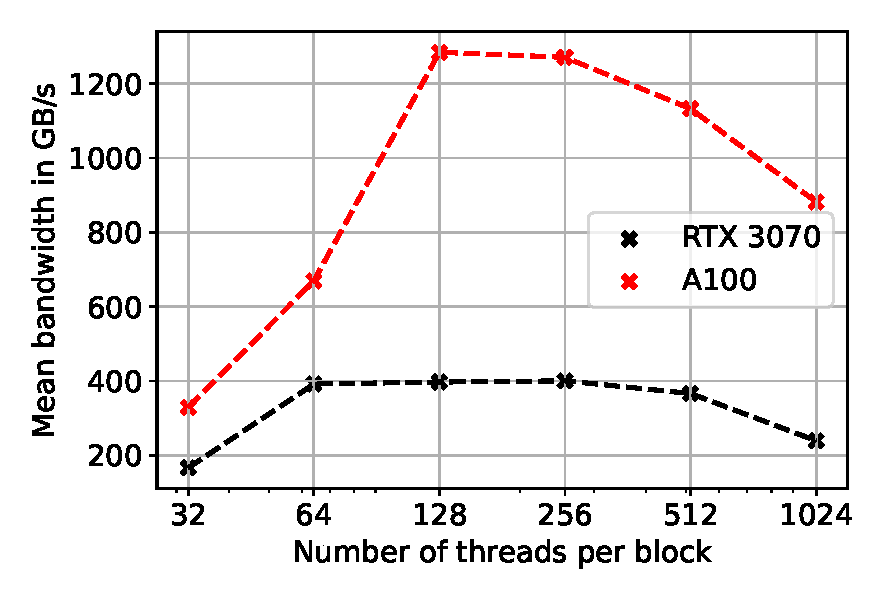
\includegraphics{num_threads.pdf}
    \caption{
        Benchmarks of the optimised kernel for \( 2^{27} \) 32-bit integers on a RTX 3070 (black) and A100 (red) for different number of threads per block.
        While the A100 outperformes the RTX 3070 as expected, they show they same characteristic in respect to the number of threads per block.
        The optimum lies somewhere between 128 and 256 threads.
    }
\end{figure}

The choice of the number of threads can have a massive impact on the performance of the application.
Usually, the optimum cannot be predicted theoretically as this becomes unfeasably complex even for simple code.
Different algorithms behave differently and it is hard to make a general statement about the optimum.
An expected behaviour, however, is the divergence for a low number of threads per block.
Here, the parallelisation overhead becomes very large and the hardware occupancy low.

The best way to approach this problem is to do test-runs of the desired calculation to find the optimum and the commit to the choice.
In our case, the optimum lies between 128 and 256 threads for both the RTX 3070 and the A100.
For the rest of the benchmarks we will therefore use 256 threads per block.

\section{Scaling of the performance towards larger and smaller array sizes}

\begin{figure} \label{fig_scaling}
    \centering
    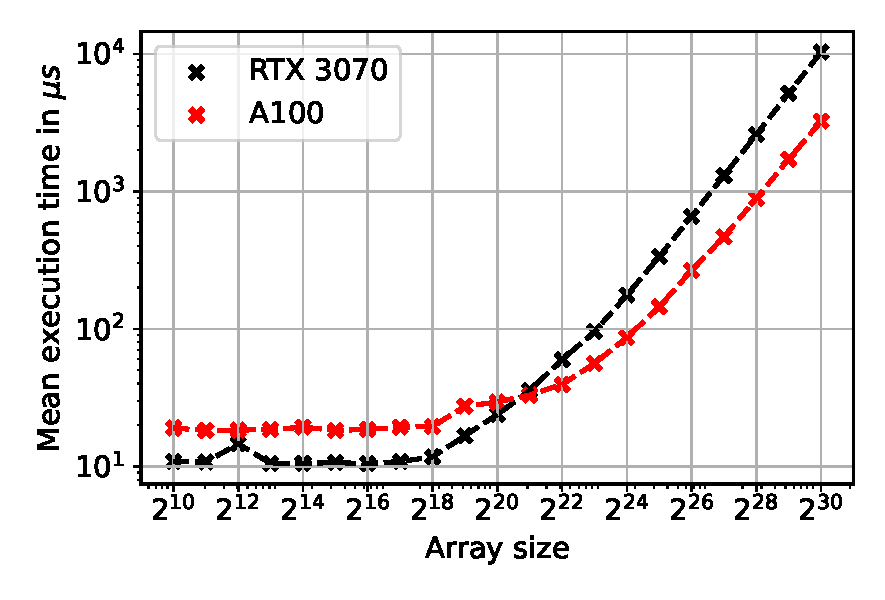
\includegraphics{scaling.pdf}
    \caption{
        Performance of the reduction kernel over increasing 32-bit array sizes for a RTX 3070 and an A100.
        All points represent the mean of 1000 measurements.
        One can see nicely the transition to linear scaling.
    }
\end{figure}

Oftentimes, the GPUs only start to be effective for large problem sizes.
This behaviour is depicted in fig. \ref{fig_scaling}.
The expected linear scaling in problem size is only achieved after a certain threshold.
The cause of this is most likely host code overhead, parallelisation overhead and device latency.
Interestingly, the RTX 3070 performs better for small array sizes.
This might be very setup dependent, however (host memory speed, CPU, etc).

Both GPUs converge towards 92\% of their respective bandwidths (RTX 3070: 448 GBytes/s, A100: 1.555 GBytes/s).
The A100 is approximately three times faster than the RTX 3070.

\section{Dependence of the performance on the datatype}

\begin{figure} \label{fig_datatypes}
    \centering
    \includegraphics{datatypes.pdf}
    \caption{
        Performance of the reduction kernel for several datatypes over an array with \( 2^{28} \) elements on a RTX 3070 (black) and an A100 (red).
        Each data point reflects the mean of 1000 measurements.
        The execution time is proportional with the size of the datatype in the case of the RTX 3070,
        while for the A100 the larger datatypes are slightly more efficient in terms of bandwidth.
    }
\end{figure}

The execution time also dependents on the underlying datatype.
In our case this dependence is depicted in fig. \ref{fig_datatypes}.
In the case of the RTX 3070 the execution time is perfectly proportional to the bit size of the datatype.
This is expected as the reduction algorithm is bottlenecked by bandwidth.
Interestingly, this behaviour is not so trivial for the A100.
The A100 is slightly more efficient for the larger datatypes, int64 and double, than for the smaller ones, int32 and float.
This can be explained by the purpose of the A100 as a scientific GPU.
The A100 is specialized on double precision calculations, while the RTX3070's purpose - as a consumer grade GPU - is to be an all-rounder \cite{programming_guide}.

\section{Conclusion}
The most important learning from the benchmarks is that the presented implementation of tree reduction is able to achieve top performance on two different Nvidia platforms.
This shows that the optimisations have a good level of generality. 
What could not be shown is the applicability of these techniques to platforms of other GPU designers, like AMD, and could be an interesting topic for future work.
However, AMD uses a similar runtime and framework to CUDA and the GPUs have similar architectures.
Therefore, one could assume that the same optimisations hold.


\printbibliography

\end{document}
